\documentclass[a4paper]{article}

\usepackage[francais]{babel}
\usepackage[utf8]{inputenc}
\usepackage[T1]{fontenc}
\usepackage[french,lined,boxed,commentsnumbered]{algorithm2e}
\usepackage{amsmath}
\usepackage{amsfonts}
\usepackage{amssymb}
\usepackage{placeins}
\usepackage{listings}
\usepackage{color}
\usepackage{textcomp}

%----- Package français
\usepackage[utf8]{inputenc} %reconnaissance des accents
\usepackage[francais]{babel} %document en français
\usepackage[T1]{fontenc} %codage des fonts TeX ?

%----- code ex: \BlankLine
\usepackage[french,lined,boxed,commentsnumbered]
{algorithm2e}


%----- math
\usepackage{amsmath}

%----- images
\usepackage{graphicx}

\title{Vérification formelle de site web\\premier rapport}
\author{Thomas BRIEN}
\date{19 Novembre 2012}

\begin{document}
\maketitle
\section{Passage du site web au graphe associé:\\}


\subsection*{ Les noeuds du graphe (documents du site)\\ }
 On défini un noeud N du graphe comme suit: N = <u, lab, loc, site, ext, Sem>\\
 avec:\\
 $u$, l'URI associée à la page\\
 $lab$, la liste des "ancres" de la page\\
 $loc$, la liste des liens locaux dans la page\\
 $site$, la liste des liens du site définis dans la page\\
 $ext$, la liste des liens externes définis dans la page\\
 $Sem$, liste d'informations représentant les informations sémentiques relatives à la page.\\
 
\subsection*{ Les liens des documents\\ }
Une fois au point sur les annotations relatives à un noeud (un document) du site, on peut s'intéresser à l'expression des liens.\\
Soit un document $s = doc(m,h,u)$ qui pointe vers un autre document $d = doc(m,h,p)$ du site:\\
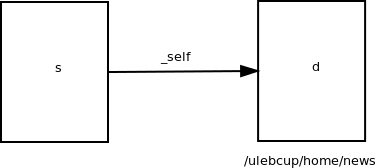
\includegraphics[scale=0.6]{lienSimple.png}\\
Un tel lien est représenté par un tuple <p, l, t>. Si le document s contient le lien html suivant:\\
<a href="/ulebcup/home/news"> News </a>\\
notre tuple devient: <p, l, t> = <"/ulebcup/home/news","", $\_$self> $\in$ site\\
$NB$: pour les liens externes, on doit repréciser la méthode et l'hote, de sorte que notre tuple sera enrichi comme suit: <m', h', p, l, t> = <"http","http://www.euroleague.net",
"/uleb/domestic-leagues","", $\_$blank>\\
\subsection*{ Les liens du graphe\\ }
On peut maintenant construire le graph associé au site en suivant les définitions données dans l'article (3.8 et 3.9)\\
\section*{ Vérification des propriétés \\ }
La vérification sera basée sur la logique LTL et appliquée à des structures de Kripke, comme défini en $page$ $9$.\\
\subsection*{ L'utilisation de la sémantique }
On s'appuie sur la sémantique des pages, de sorte que chaque élément de l'ensemble $Sem \mid_2$ peut être vu comme une propriété atomique. On peut par exemple écrire une formule qui vérifie que les pages privées ne sont pas accessibles directement depuis les pages publiques. On résonne sur $Sem$ = <"scope": \{public, private, access\}>: $\neg(public U private)$. En effet, on doit vérifier la propriété access avant de pouvoir vérifier private.\\
\section*{ Extensions souhaitables: }
\begin{itemize}
\item au niveau du langage (pas seulement html)
\item au niveau de la quantification du temps en LTL
\end{itemize}

\end{document}